\chapter{Subsistema de control y presentación}

\section{Introducción}

El último de los subsistemas que conforma el sistema de medida digital es
el subsistema de control y presentación. Es el subsistema de más alto nivel
de entre los que integran el sistema por interactuar directamente con el
supervisor. El subsistema de control y presentación está constituido por
los bloques de control y presentación propiamente dichos, tal y como
muestra la \cref{fig:subconpre}. Sin embargo, en la práctica estos dos
bloques se engloban en una misma entidad que en este documento se denomina
\emph{software de control}.

\begin{figure}
	\begin{center}
		\includegraphics{gis-pfc-ch3-01.mps}
	\end{center}
	\caption[Subsistema de control y presentación] {Bloques de control
	y presentación dentro del subsistema de control y presentación.}
	\label{fig:subconpre}
\end{figure}

El subsistema de control y presentación, al actuar como interfaz entre el
supervisor y el sistema de medida, debe ser capaz de poner en práctica las
órdenes que administra el supervisor y gestionar el funcionamiento del
resto de subsistemas. De entre los dos bloques que conforman el subsistema,
es el bloque de control ---como su nombre indica--- el encargado de esta
actividad. Como tal, es responsabilidad suya la ejecución de las siguientes
tareas:

\begin{itemize}
	\item Iniciar y detener la sesión de adquisición.
	\item Interactuar con los drivers de la tarjeta por medio del
		sistema operativo para controlar parámetros de la sesión de
		adquisición como pueden ser, por ejemplo, puertos de
		entrada, modos de adquisición y terminación, o frecuencia
		de muestreo.
	\item Realizar el mantenimiento de los buffers de memoria. Tarea
		que puede dividirse, o consta a su vez, de dos tareas de
		menor complejidad: dar formato a las muestras almacenadas
		en el o los buffers situados en la memoria interna de la
		tarjeta para su comprensión por parte del ordenador
		anfitrión; trasladar las muestras formateadas adecuadamente
		a la memoria del \pc{} para que de ese modo puedan ser
		manipuladas por el usuario administrador.
\end{itemize}

Por su parte, al bloque de presentación le corresponde la tarea de
presentar al supervisor información de utilidad a partir de los datos
obtenidos del subsistema de adquisición, en este caso de la señal digital.
La información debe mostrarse al supervisor de forma que este sea capaz de
interpretarla. En consecuencia, y por criterio propio, se decide por
diseñar el software de control para que sea capaz de proporcionar al
supervisor la siguiente información de la señal: % Lo de criterio propio
% significa que era uno de los objetivos del proyecto que propuso el
% director.

\begin{itemize}
	\item El valor instantáneo cada 250 ms.
	\item El valor medio en el mismo intervalo de tiempo. Este valor
		debe calcularse a partir de las muestras obtenidas en dicho
		periodo a una frecuencia de muestreo que queda a elección
		del supervisor. Debe ser posible seleccionar la frecuencia
		de muestreo desde el propio software de control.
	\item La forma instantánea de la señal, de un fragmento de una
		duración determinada. Debe ser posible también seleccionar
		la duración del fragmento. Simultáneamente debe
		representarse el espectro en frecuencia del fragmento de
		señal que aparece en pantalla.
\end{itemize}

Se impone una condición de diseño adicional al software de control, debe
ser poco exigente con respecto al \pc{} anfitrión en cuanto a capacidad de
procesado y memoria principal utilizada. Para lograrlo se propone la
siguiente solución: en lugar de mostrar al mismo tiempo el valor
instantáneo de la señal, el valor medio, y su forma, se concibe la
aplicación para que el usuario pueda elegir uno de estos tres aspectos de
la señal y sólo ese se muestra por pantalla.

Por conveniencia se adopta la siguiente nomenclatura en este documento: se
dice que en el \emph{modo gráfico} la aplicación muestra gráficas que
representan la forma de la señal y de su espectro en frecuencia; mientras
que en los \emph{modos numéricos} o no gráficos lo que aparece en pantalla
es un valor numérico relacionado con la magnitud variable de la señal ---el
voltaje---. Aplicando de nuevo el criterio de austeridad por el cual la
aplicación debe ser lo menos exigente posible, se consigue economizar
recursos en el modo gráfico de funcionamiento si se permite al supervisor
seleccionar si son ambos, forma y espectro de la señal, los representados,
sólo uno y cual, o ninguno de ellos.


\subsection{Funcionamiento de un osciloscopio}

El objetivo primordial del software de control es implementar un modo
gráfico con el que el supervisor pueda observar cual es el aspecto de la
señal y como es su espectro en frecuencias. En el proceso previo de diseño
se considera que modelo se puede tomar como referencia para implementar el
modo gráfico. Por sus bondades, se elige el osciloscopio digital. En la
representación de señales el instrumento empleado en la mayoría de
aplicaciones es el osciloscopio digital. Los osciloscopios son instrumentos
prácticos que permiten visualizar señales de forma efectiva.

Para tratar de imitar el funcionamiento del osciloscopio digital en el
software de control, es preciso conocer como funciona este dispositivo y
cuales son sus características principales. Como parte de este capítulo se
ha querido proveer una introducción al comportamiento de los osciloscopios
digitales que se extrae del estudio realizado sobre estos dispositivos al
acometer este episodio del proyecto fin de carrera. Se expone esencialmente
de que forma consigue el osciloscopio representar la señal, como lo hace.
Para ello se documentan los distintos modos de representación de que cuenta
el osciloscopio digital en comparación con su equivalente analógico. De ese
modo el lector que acuda a esta introducción al comportamiento de los
osciloscopios digitales puede formarse una imagen del aspecto que debe
tener el software de control, lo que sirve a dos propósitos diferentes:

\begin{itemize}
	\item El primero y más inmediato, permitirle ubicar de forma muy
		precisa los objetivos del proceso de programación. De forma
		que le sea posible identificar, en cierto modo, que rutinas
		son necesarias para lograr el resultado final.
	\item Y además puede servirle como nota introductoria al
		\cref{chap:part1conclusions} en el que se comparan los
		resultados obtenidos en un experimento realizado primero
		mediante el sistema digital de medida y, posteriormente,
		utilizando un osciloscopio digital en conjunción con el
		subsistema para la interacción con el medio físico.
\end{itemize}


\subsection{Osciloscopios analógicos, osciloscopios digitales y retardo}

Los osciloscopios analógicos emplean un tubo de rayos catódicos y un
monitor de fósforo para generar una imagen de la señal. El cursor que el
tubo dibuja en el monitor lo va barriendo de izquierda a derecha con
periodicidad, y su posición vertical refleja a cada momento el valor de
tensión de la señal eléctrica que entra al osciloscopio. El monitor
preserva durante breves instantes una traza del cursor y así se forma la
imagen que representa a la señal.

En la actualidad los osciloscopios analógicos están siendo desplazados en
su uso por los osciloscopios digitales. El procedimiento que sigue un
osciloscopio digital para representar señales es completamente diferente al
que siguen los osciloscopios analógicos. Constantemente el osciloscopio
digitaliza la señal en seguimiento, procesa la señal digital resultante y
la almacena en memoria. Cada cierto \emph{periodo de refresco} el
osciloscopio muestra por pantalla una representación de los datos que
previamente ha almacenado durante ese mismo periodo. Mientras se recogen
datos para una nueva imagen se mantienen en pantalla los datos
correspondientes al periodo anterior. La velocidad con la que se suceden
las imágenes en el monitor del osciloscopio hace que se produzca la
sensación de movimiento, y de ese modo la representación responde a las
variaciones que se producen en la señal. Esto permite observar los eventos
que se producen en la señal en determinadas situaciones, como por ejemplo:
al accionar un potenciómetro que forma parte de un circuito que está siendo
analizado, al cambiar la configuración de un generador de señales para que
genere una señal diferente a la que suministraba unos instantes antes, o
simplemente al conectar la alimentación.

El periodo de refresco no es fijo, de lo contrario los datos mostrados en
el monitor del osciloscopio aparecerían en exceso comprimidos o expandidos
en función de la frecuencia de la señal monitorizada. Puede configurarse el
periodo de muestreo para que adopte un valor de entre un rango de valores
predeterminados. Debe notarse que al ser posible modificar el valor del
periodo de refresco existe la posibilidad de que, en efecto, éste adopte un
valor alto. Ésto haría que el retardo que se produce en la sucesión de
imágenes aumentase, limitando la capacidad de la representación de seguir
los cambios que afectan a la señal. Para impedir que ésto ocurra los
osciloscopios digitales implementan un mecanismo por el cual una señal se
representa de uno u otro modo en función del valor que toma el periodo de
refresco.

% >>|Fecha indeterminada|
%
%	Un periodo de refresco demasiado alto puede ser la causa de un
%	retardo excesivo en la sucesión de imágenes, haciendo que la
%	representación de la señal reaccione con lentitud a las variaciones
%	que en ésta última se produzcan.
%
%	No existe ningún cursor, se generan fotogramas de la señal en
%	seguimiento\footnote{En realidad los osciloscopios digitales
%	modernos disponen de más de un canal de entrada y por tanto pueden
%	representar por pantalla varias señales simultáneamente.}, imágenes
%	que muestran la representación de un fragmento de la señal y que
%	cubren la pantalla del osciloscopio por completo. Una vez aparece
%	una imagen por pantalla permanece estática hasta que una nueva
%	imagen la sustituye. Al sucederse las imágenes rápidamente en la
%	pantalla del osciloscopio se produce una sensación de movimiento, y
%	la representación responde a las variaciones que se producen en la
%	señal.
%
%	El periodo de tiempo que transcurre entre dos imágenes puede
%	identificarse como \emph{periodo de refresco}. El periodo de
%	refresco está estrechamente relacionado con la duración temporal
%	del fragmento de señal que se representa por pantalla. La señal
%	monitorizada se desconoce de antemano, por tanto, para representar
%	un fragmento de una duración determinada el osciloscopio debe
%	esperar hasta reunir la suficiente información. Esto no ocurre con
%	los osciloscopios analógicos puesto que éstos representan la señal
%	en tiempo real.
%
%	Como en cualquier osciloscopio analógico un usuario debería ser
%	capaz de configurar un osciloscopio digital para que represente los
%	datos correspondientes a un periodo de tiempo más o menos largo. De
%	lo contrario, supondría una gran dificultad para el seguimiento de
%	señales cuya frecuencia difiriese en gran medida con el periodo de
%	refresco.
%
%	La posibilidad de ajustar el periodo de muestreo presenta un
%	inconveniente relacionado con el modo de funcionamiento de los
%	osciloscopios digitales.
%
%	Debe notarse que al existir la posibilidad de ajustar el periodo de
%	refresco, existe la posibilidad. Debe notarse que al utilizar un
%	periodo de refresco de valor variable.
%
%	Lo que yo veo es que si puedo ajustar el periodo de refresco al
%	valor que yo quiera dentro de un rango predeterminado puedo hacer
%	que sea demasiado alto y eso causa el retardo y que no se pueda
%	seguir fácilmente los eventos que se producen en la señal. Debe
%	tenerse en cuenta. Debe notarse.
%
%	LO IMPORTANTE AQUÍ ES EXPLICAR POR QUÉ LOS DATOS SALEN COMPRIMIDOS
%	O EXPANDIDOS SI EL PERIODO DE REFRESCO ES FIJO (Esto no es
%	necesario, el lector debe tener los conocimientos necesarios para
%	saber que si la frecuencia de la señal aumenta y el periodo de
%	refresco es el mismo y las dimensiones de la pantalla son las
%	mismas la representación de la señal aparecerá más comprimida)
%
%	Los controles del osciloscopio digital deben permitir al usuario
%	del osciloscopio ajustar el periodo de refresco.
%
%	En ocasiones es preciso.
%
%	Para poder trabajar con señales de frecuencias altas o bajas que
%	difieran en gran medida de la frecuencia con la que se refresca el
%	monitor del osciloscopio es preciso poder modificar el periodo de
%	refresco.
%
%	Para poder trabajar correctamente con señales cuya frecuencia
%	difiera en gran medida de la tasa de refresco del monitor del
%	osciloscopio es preciso.
%
%	Que exista la posibilidad/poder modificar/variar/alterar dicha
%	tasa/el periodo de refresco.
%
%	Debe poder modificarse.
%
%	Si el periodo de refresco toma un valor muy alto y nada lo impide
%	el retardo que se produce entre .
%
%	Puede producir/es causa  que ocurre en el monitor del osciloscopio.
%	Para impedir que ésto ocurra/este fenómeno ocurra/se produzca los
%	osciloscopios digitales implementan un mecanismo.
%
%	Por el cual alteran el modo en que una señal se representa en
%	función del valor que toma el periodo de refresco.
%
%	Cada dos imágenes/cada imagen.
%
%	Por suerte. Implementa un mecanismo.
%
%	Para poder trabajar con señales de frecuencias altas o bajas que
%	difieran en gran medida de la frecuencia con la que se refresca el
%	monitor del osciloscopio debe ser posible modificar el periodo.
%
%	El aspecto que muestra la pantalla de un osciloscopio digital en un
%	instante determinado se.
%
%	El resultado es una imagen. La imagen que aparece en pantalla.
%
%	Para resolver los problemas provocados por señales.
%
%	Para evitar algunos de los problemas que en los osciloscopios
%	analógicos provocaban las señales lentas o las señales rápidas
%	(mentira, el problema es barrer la pantalla con el cursor y el
%	osciloscopio ya lo resuelve per se).
%
%	Dado que el usuario puede modificar la duración de los fragmentos
%	de señal que aparecen por pantalla podría producirse una situación
%	en la que la duración del fragmento es demasiado prolongada el
%	retardo que se produce entre dos imágenes conduce a que el desfase
%	entre la señal y la información representada en pantalla sea
%	notable.
%
%	El usuario puede modificar la duración del eje temporal de la
%	representación --> luego, si la representación ocupa por completo
%	el monitor del osciloscopio, lo que cambia es la duración de los
%	fragmentos. Voy a clarificar la relación anterior, el eje de
%	tiempos es siempre de la misma longitud, sin embargo no siempre
%	representa la misma cantidad de tiempo. El usuario puede hacer que
%	represente un tiempo mayor o un tiempo menor. Si representa un
%	tiempo mayor entonces el fragmento de señal necesario para cubrir
%	el eje de tiempos es mayor y se necesita más tiempo para
%	adquirirlo. El objeto de que pueda modificar la duración del eje
%	temporal es que pueda observar detalles que no se pueden apreciar
%	de otra manera, o seguir señales de menor frecuencia.
%
%	Dado que la duración de los fragmentos puede seleccionarse.
%	Puede/Podría producirse una situación. Esta situación es
%	inconveniente.
%
%	Pese a las mejoras que los osciloscopios han experimentado desde su
%	aparición, como por ejemplo la capacidad de los osciloscopios
%	digitales de medir ciertos parámetros de una señal como su periodo
%	o su valor de pico a pico, el propósito original de estos
%	dispositivos es el de mostrar el aspecto de una señal de forma que
%	pueda extraerse de éste cualquier información que pudiera deducirse
%	de él. % Pueda extraerse cualquier información de la señal que
%	pudiese deducirse a partir de su apariencia.
%
%	En este sentido un osciloscopio debe mostrar una imagen de la señal
%	actual y permitir al usuario modificar aspectos de la
%	representación como la escala con la que se representan las
%	tensiones.
%
%	La dimensión temporal de la representación determina cuanto debe
%	esperar el osciloscopio desde que se muestra por pantalla una
%	imagen hasta que se puede generar la siguiente. El retardo que se
%	produce es la consecuencia de representar de una vez un fragmento
%	de una duración determinada de una señal que se desconoce de
%	antemano. Al contrario que ocurre con los osciloscopios analógicos
%	que representan la señal en tiempo real, los osciloscopios
%	digitales deben esperar hasta reunir la suficiente información de
%	la señal. En otras palabras, aparece un retardo que depende
%	exclusivamente de la duración del fragmento de señal necesario para
%	cubrir la ventana del osciloscopio, o lo que es lo mismo, el
%	retardo es independiente de otros parámetros como son la velocidad
%	de muestreo o la potencia de procesado del osciloscopio.\par
%
%	Este modo de proceder tiene un inconveniente, el objetivo de un
%	osciloscopio es mostrar en cada momento como es la forma de la
%	señal, si el retardo introducido es demasiado alto el osciloscopio
%	deja de ser eficaz pues la información que proporciona cada imagen
%	es obsoleta. Problema que se ve agravado por la posibilidad de
%	configurar el eje de tiempos. Tanto los osciloscopios analógicos
%	(variando la frecuencia de barrido del cursor) como los
%	osciloscopios digitales, permiten que el usuario modifique la
%	cantidad de tiempo que refleja el eje horizontal de la
%	representación, pudiendo ser ésta mayor o menor. A efectos
%	prácticos, en los osciloscopios digitales el tiempo abarcado por el
%	eje temporal actúa como el inverso de la frecuencia de refresco del
%	monitor, por tanto, cuanto mayor sea ese tiempo con mayor lentitud
%	se sucederán las imágenes y habrá un mayor desfase entre la señal y
%	la representación de ésta.
% <<<


\subsection{Modos de representación en los osciloscopios digitales}\label{subsec:repmodes}

%	Los osciloscopios digitales tienen la capacidad de representar una
%	señal de dos formas diferentes: una en la que la señal aparece
%	anclada a la ventana del osciloscopio, que en este documento se ha
%	asociado al nombre \emph{modo disparado}; y otra en la que la señal
%	se desplaza de derecha a izquierda en la pantalla del osciloscopio,
%	que aquí se conoce como \emph{modo continuo}.

Los osciloscopios digitales tienen la capacidad de representar una señal de
formas diferentes. Cada forma de representar la señal se conoce en este
documento como \emph{modo de representación}. Habitualmente los
osciloscopios digitales cuentan al menos con dos modos de representación.
Estos dos modos son, tal y como han sido bautizados aquí, el \emph{modo
disparado} y el \emph{modo continuo}. Los modos de representación continuo
y disparado forman parte de la solución que los osciloscopios digitales
adoptan para combatir la situación hipotética en la que un excesivo retardo
entre cuadros pudiese complicar el seguimiento de la señal.

Para evitar las consecuencias de un retardo alto, un osciloscopio digital
conmuta al modo de representación continuo cuando el periodo de refresco
supera los 200 ms, el resto del tiempo permanece en el modo de
representación disparado. % Para remediar el retardo, un osciloscopio
% digital conmuta al modo de representación continuo cuando el periodo de
% refresco supera los 200 ms, el resto del tiempo permanece en el modo de
% representación disparado.

Para evitar las limitaciones que el modo de representación disparado
presenta en configuraciones en las que el periodo de refresco toma un valor
elevado, un osciloscopio conmuta al modo de representación continuo en el
caso en el que el periodo de refresco supere los 200 ms. Habitualmente el
osciloscopio digital opera en el modo de representación disparado, que es
el modo que responde a la descripción funcional que se ha hecho de los
osciloscopios digitales en este apartado.

% >>|Miércoles 1 de Diciembre de 2010|
%
%	El modo de representación disparado es el modo de representación
%	por defecto/que el osciloscopio emplea por defecto. Hasta ahora el
%	concepto era que el osciloscopio digital empleaba un modo de
%	representación para mostrar los datos por pantalla, el nuevo
%	concepto es que los datos se representan de uno u otro modo.
%
%	Una razón para poner el límite en 200 ms es que de ese modo puede
%	salir por pantalla un periodo entero de una señal de 5 Hz, en
%	realidad algo menos de un periodo con esa frecuencia. Eso no quiere
%	decir que el osciloscopio pueda disparar señales de menor
%	frecuencia con esa configuración del periodo de refresco. De hecho,
%	podría disparar señales con una frecuencia mínima de 1 Hz o 2.
%
%	Creo que podría resolver esta introducción a los modos de
%	representación de los osciloscopios digitales del siguiente modo.
%	En primer lugar menciono como hago que existen dos modos básicos de
%	representación que están presentes en cualquier osciloscopio
%	digital. Digo que esos dos modos forman parte de la solución que
%	los osciloscopios adoptan para evitar los problemas que derivan de
%	una configuración en la que el tiempo de refresco adopta un valor
%	demasiado alto. Después paso a decir que el osciloscopio evita el
%	problema al cambiar a un modo de representación que no se ve
%	afectado por el periodo de refresco cuando éste toma un valor alto.
%	Como valor alto se entiende cualquiera superior a los 200 ms, el
%	límite se escoge en 200 ms porque la representación en modo
%	disparado es más adecuada para seguir las variaciones que se
%	producen en la señal pero sólo permite representar señales cuyo
%	periodo sea similar al periodo de refresco, por tanto, señales cuyo
%	periodo sea superior a los 200 ms sólo podrán observarse
%	(correctamente) en el modo de representación continuo.
% <<<
%
% >>|El modo disparado|
%
%	El modo disparado es el que responde a la descripción funcional que
%	se ha dado hasta el momento de los osciloscopios digitales. En este
%	modo un osciloscopio digital puede imitar a un osciloscopio
%	analógico. En este modo la representación de la señal aparece
%	anclada a la ventana del osciloscopio. De hecho disparar la señal
%	viene a decir fijarla en una posición concreta de la ventana. Para
%	conseguirlo el osciloscopio debe poder determinar donde se
%	encuentran los cruces de la señal con respecto a un nivel de
%	umbral. Una vez localizados la representación puede desplazarse
%	según un criterio que habitualmente se deja en manos del
%	supervisor.
% <<<
%
% >>|Martes 23 de Noviembre de 2010|
% 
% 	A continuación las palabras que he consultado hoy para incluir en
% 	la memoria.
% 
% 	He consultado la palabra \emph{evento}, por que en párrafos
% 	anteriores he escrito algo como «esto permite observar los eventos
% 	que se producen en la señal en determinadas situaciones», y no me
% 	quedaba del todo claro lo que quería decir. Pensaba que tal vez los
% 	eventos no se producían en la señal, que las consecuencias del
% 	evento eran las que se reflejaban en la señal. Por poner un
% 	ejemplo: si yo actúo sobre un potenciómetro, el evento es que el
% 	valor de la resistencia que se observa en bornes del potenciómetro
% 	ha cambiado, la consecuencia reflejada en la señal puede ser un
% 	cambio en el voltaje de pico a pico, un cambio de forma, un cambio
% 	en la frecuencia.., todo depende del circuito que influye en la
% 	señal. Sin embargo, esto no es del todo cierto porque un evento es
% 	cualquier cosa que sucede y producir es ocasionar, es decir, que si
% 	cambia el voltaje de pico a pico de la señal es una cosa que sucede
% 	en la señal. Evento es lo mismo que acaecimiento o cosa que sucede.
% 	Producirse es lo mismo que originarse o ocasionar.
% 
% 	El verbo responder también me intriga en el siguiente contexto:
% 	«este umbral responde a una solución de compromiso». El significado
% 	más probable en este contexto según mi opinión puede ser el
% 	siguiente: «RAE 13. intr. Dicho de una cosa: Tener proporción,
% 	corresponder con otra». Podría traducirse la expresión original en
% 	«este umbral es una solución de compromiso».
% <<<
% 
% >>|Anteriores al 23 de Noviembre de 2010|
%
% 	Para combatir el retardo que se produce en
% 	configuraciones/situaciones en las que el periodo de refresco es
% 	muy alto Este límite responde a una solución de compromiso.  Para
% 	determinar el umbral se hace caso a dos criterios/factores se
% 	tienen en cuenta/la influencia
% 
% 	Dos factores influyen en la elección del umbral o límite o.  De
% 	momento lo único que tengo dicho es que: para evitar las
% 	consecuencias de un retardo alto el osciloscopio conmuta al modo
% 	continuo cuando el periodo de refresco <<supera>> los 200 ms; y que
% 	la elección del umbral no es trivial. Lo que me queda por decir es
% 	mucho: tengo que dar un motivo por el cual se haya elegido 200 ms
% 	como referencia en la que se conmuta los modos, las ideas están
% 	abajo, poder ver periodos completos de señales de frecuencia muy
% 	baja (5 Hz) con el modo continuo, y que el retardo no impida el
% 	correcto seguimiento de la señal. El problema es que al no haber
% 	explicado por qué el modo continuo no acusa los defectos del modo
% 	disparado (como refresca la pantalla al completo no existe
% 	correlación entre el periodo de refresco y la dimensión de la
% 	ventana, entonces el retardo no es aplicable), y que no representa
% 	periodos de la señal completos (no es eso, si no que no es tan
% 	bueno para apreciar los cambios que se producen en la señal); no
% 	puedo justificar bien por qué el límite en 200 ms. También puedo
% 	decir algo como: <<todo cobrará sentido más adelante>>, <<podrá
% 	comprenderse esta elección al terminar el apartado>>. Aunque claro
% 	no me gusta escribir las cosas en futuro y utilizar otras partes de
% 	la memoria para dar pie a lo que estoy diciendo.
% 
% 	La elección del límite/umbral en el que el osciloscopio conmuta
% 	entre uno u otro modo no es trivial. Este límite responde a un
% 	compromiso por el cual se consigue representar señales de
% 	frecuencia tal sin que el retardo suba.  Deben considerarse dos
% 	factores: En primer lugar/primeramente, está poder representar
% 	señales de frecuencias bajas Este límite responde a un compromiso
% 	entre el retardo y la apariencia de los datos. Que busca evitar en
% 	la mayor medida posible las consecuencias de los altos retardos al
% 	mismo tiempo que Este límite responde a un compromiso Que por un
% 	lado consigue que puedan seguirse Dada la peculiaridad con la que
% 	se representa una señal en el modo continuo, la representación en
% 	este modo no se ve afectada por el periodo de refresco.  Complacer
% 	El compromiso es entre que se vean periodos de señales lentas y que
% 	el retraso no sea demasiado.
% 
% 	El mayor retraso que se produce entre un cambio en la señal y la
% 	subsecuente aparición del mismo en la pantalla del osciloscopio
% 	será de 200 ms, lo cual no es mucho, y a pesar de que el ojo lo
% 	aprecia, tampoco es demasiado grave. Por otro lado si el periodo de
% 	refresco es de 200 ms puede apreciarse en la pantalla del
% 	osciloscopio un periodo completo de señales de hasta unos 5 Hz. Un
% 	compromiso por el cual el osciloscopio se compromete a dar servicio
% 	de una determinada calidad. Un compromiso entre el retardo y la
% 	apariencia de los datos.
% 
% 	Aquí me sale la complicación de explicar que en el modo continuo
% 	aunque el eje de tiempos cubre un determinado intervalo, este no se
% 	corresponde con el periodo de refresco. Pero esto podría reservarlo
% 	para el punto en el que trato el modo de representación continuo.
% 	El modo de representación disparado debería explicarse al
% 	principio, ya que en este modo la señal se representa como lo hacen
% 	los osciloscopios analógicos y, además, todo lo que se ha dicho
% 	sobre como representa la señal un osciloscopio digital hace
% 	referencia a este modo. El modo disparado es el que normalmente
% 	está activado, por eso yo lo había llamado modo convencional,
% 	aparte de lo que he dicho en este párrafo sobre él.  En el modo de
% 	representación disparado los datos se representan de modo que
% 	cubren la extensión horizontal de la ventana del osciloscopio. El
% 	eje de tiempos representa pues una medida similar al periodo de
% 	refresco. Después añado que el periodo de refresco es igual al
% 	tiempo que necesito para adquirir muestras suficientes para cubrir
% 	la ventana, para adquirir muestras adicionales para corregir la
% 	posición de la señal y que no aparezcan huecos, y para procesar,
% 	almacenar y representar las muestras. En el modo de representación
% 	continuo el eje de tiempos de la ventana del osciloscopio
% 	representa un periodo de tiempo que siempre es mayor que el periodo
% 	de refresco y en ocasiones mucho mayor. De ese modo cuando la
% 	imagen se refresca no desaparecen todos los datos si no que se van
% 	desplazando.
% 
% 	La necesidad de disponer de dos modos de representación surge como
% 	parte de una solución al problema Expuesto en el punto
% 	anterior/ocasionado por.
% 
% 	Para evitar los altos retardos que se producen en configuraciones
% 	en las que el periodo de refresco es muy bajo. Los altos retardos
% 	que se producen en configuraciones del periodo de refresco muy
% 	bajo. En configuraciones en las que el periodo de refresco es muy
% 	bajo.
% 
% 	Y surgen como parte de una solución al problema expuesto en el
% 	punto anterior ocasionado por.
% <<<


\subsubsection{Criterios para la selección del modo}

%	Existen dos modos de representación. Por lo general se toma como
%	criterio utilizar el modo de representación disparado cuando el
%	periodo de refresco es inferior a los 400 ms. Se toma como
%	criterio, ¿qué es un criterio? Criterio = Discernimiento = Acción y
%	efecto de discernir; Discernir = Distinguir algo de otra cosa,
%	señalando las diferencias que hay entre ellas.
%
%	Es decir, se toma criterio para discernir entre las situaciones en
%	las que es conveniente representar la señal de uno u otro modo.

Para evitar que en determinadas configuraciones del eje temporal del
osciloscopio el retardo sea excesivo, la mayoría de estos dispositivos
implementan dos modos de funcionamiento: el modo convencional que se aplica
en situaciones en las que el retardo no se considera importante; y una
especie de modo continuo. Existen dos criterios que se siguen de manera
habitual para diferenciar en que momento es más apropiado el uso de uno u
otro modo.


\subparagraph{Criterio de animación}

El primer criterio evalúa el correcto funcionamiento del modo convencional.
El modo convencional de representación en un osciloscopio requiere que la
cantidad de imágenes que salen por pantalla cada segundo sea lo suficiente
grande como para que se simule el movimiento. Por tanto para satisfacer el
primer criterio, la tasa de refresco del monitor del osciloscopio debe
superar las veintiséis imágenes por segundo o encontrarse alrededor de esta
cifra.


\subparagraph{Criterio de disparo}

El segundo criterio está relacionado con la función de disparo que se da en
el modo convencional de representación. Para poder efectuar correctamente
el disparo sobre señales de baja frecuencia, al generar cada imagen el
osciloscopio debe haber registrado al menos un ciclo de la señal
pertinente\footnote{En la práctica se necesita algo más de un ciclo de una
señal para poder garantizar el correcto disparo de ésta. Sin embargo, es
común conseguir disparar una señal aunque la configuración del eje de
tiempos del osciloscopio permita sólo obtener una fracción del ciclo
completo de esa señal durante la realización de cada imagen.}. Lo cual
reduce la tasa mínima de refresco a la frecuencia de la señal más lenta que
se desee representar de forma correcta en el modo convencional de
representación del osciloscopio.

Como puede verse el segundo criterio es más restrictivo pues depende de la
frecuencia de la señal y ésta puede ser en efecto inferior a un hercio, es
por ello que se emplea habitualmente. Siendo así, la tasa de refresco
mínima que se permite en el modo convencional en la gran mayoría de
dispositivos y que se ha adoptado para el software de control, es de cinco
imágenes por segundo (5 Hz). Cuando se configura un osciloscopio en el modo
convencional para que trabaje a esta tasa de refresco es habitual poder
visualizar señales de frecuencia cercana a 1 Hz, sin embargo la
representación se optimiza para configuraciones en las que el osciloscopio
muestra, al menos, veinticinco imágenes por segundo, lo cual es apropiado
para señales con una frecuencia mínima de 50 Hz. Si la configuración del
eje de tiempos del osciloscopio obligara al dispositivo a trabajar con una
frecuencia de refresco inferior a la especificada, automáticamente conmuta
para funcionar en el modo continuo.


\subsubsection{Modos de representación}

Una vez visto cual es la frecuencia umbral a la que el dispositivo conmuta
entre los dos modos, debe explicarse que diferencia un modo de
funcionamiento de otro. Para ello se expone a continuación cuales son los
fundamentos de uno y otro modo.


\subparagraph{Modo continuo}

La representación en \emph{modo continuo} es, por decirlo así,
ininterrumpida. La imagen de la señal de interés se desplaza de derecha
izquierda a medida que transcurre el tiempo. Para lograr este efecto se
aumenta la frecuencia de refresco a expensas de que, como es sabido, el
fragmento de señal obtenido para cada imagen no puede cubrir la pantalla al
completo. Ocurre así por que la frecuencia de refresco es muy alta para el
eje temporal, que en este caso representa un periodo tiempo relativamente
alto. Por consiguiente, en el intervalo en el que una imagen de la señal da
paso a la siguiente en la ventana del osciloscopio, no transcurre el tiempo
suficiente como para captar un fragmento de señal de duración igual a la
abarcada por el eje de tiempos.

Las figuras \cref{fig:freesignalcont,fig:modconti} muestran con detalle
estos aspectos del modo de representación continuo. En la
\cref{fig:freesignalcont} aparece la señal que entra en el osciloscopio, se
muestran además unas marcas de tiempo que indican los instantes en los que
la imagen que muestra el osciloscopio cambia\footnote{Se ha considerado el
\emph{periodo de refresco} de la ventana del osciloscopio igual a la suma
de la \emph{ventana de adquisición} y un \emph{periodo de inactividad} en
la adquisición ocupado por el procesado de las muestras. La ventana de
adquisición es equivalente a la cantidad de tiempo que el sistema necesita
para adquirir un fragmento de señal suficiente para cubrir una porción del
eje de tiempos (en el caso del modo de funcionamiento continuo) o para
cubrir el eje de tiempos por completo más las muestras de descarte (en el
modo disparado). El periodo de inactividad es igual al tiempo requerido
para procesar el fragmento de señal adquirido en el espacio de una ventana
de adquisición.}. La \cref{fig:modconti} muestra cual es el aspecto del
osciloscopio en dos instantes posteriores al instante inicial en el que
empieza a monitorizarse la señal.

\begin{figure}
	\begin{center}
		\includegraphics{gis-pfc-ch3-04.mps}
	\end{center}
	\caption[Fragmentos de señal ordenados según el orden en el que
	llegan al sistema]{Fragmentos de señal ordenados según el orden en
	el que llegan al sistema. Cada instante marcado se encuentra
	separado de los adyacentes por un periodo de refresco. Debe
	recordarse que el modo de funcionamiento continuo se emplea en la
	monitorización de señales lentas, por lo que el periodo de
	inactividad es en este caso despreciable frente a la duración de la
	ventana de adquisición.}
	\label{fig:freesignalcont}
\end{figure}

\begin{figure}
	\begin{center}
		\includegraphics{gis-pfc-ch3-05.mps}
	\end{center}
	\caption[Dos líneas de prueba]{Dos líneas de texto de prueba para
	comprobar como cambia la estructura del documento si lo comprimo un
	poquito.}
% 	\caption[<++>]<++>{}<++>
% 	\caption[Modo de funcionamiento continuo]{Puede observarse como la
% 	llegada de un nuevo fragmento de señal al sistema en el instante
% 	$t_2$ desplaza el fragmento previamente representado en la ventana
% 	del osciloscopio una periodo de refresco a la derecha.}
	\label{fig:modconti}
\end{figure}

En el instante $t_1$ el fragmento de señal que se ha digitalizado aparece
en el extremo derecho de la representación, el resto se deja en blanco. En
cada nuevo fotograma se desplazan los fragmentos de señal representados
hasta el momento el suficiente espacio hacia la izquierda como para
incorporar un nuevo fragmento de señal. Así la porción de señal
representada aumenta cada vez más hasta que el extremo izquierdo de la
figura alcanza el margen izquierdo de la ventana del osciloscopio. Cuando
esto ocurre, empieza un desplazamiento cíclico, al incorporar un nuevo
fragmento de señal a la derecha se retira un fragmento de la misma
proporción temporal al otro extremo. Este fenómeno bien puede observarse en
la \cref{fig:modcontii}, en el ejemplo el eje temporal es equivalente a
cinco ventanas de adquisición, la llegada de un sexto fragmento de señal al
sistema conduce al inicio de la representación cíclica.

\begin{figure}
	\begin{center}
		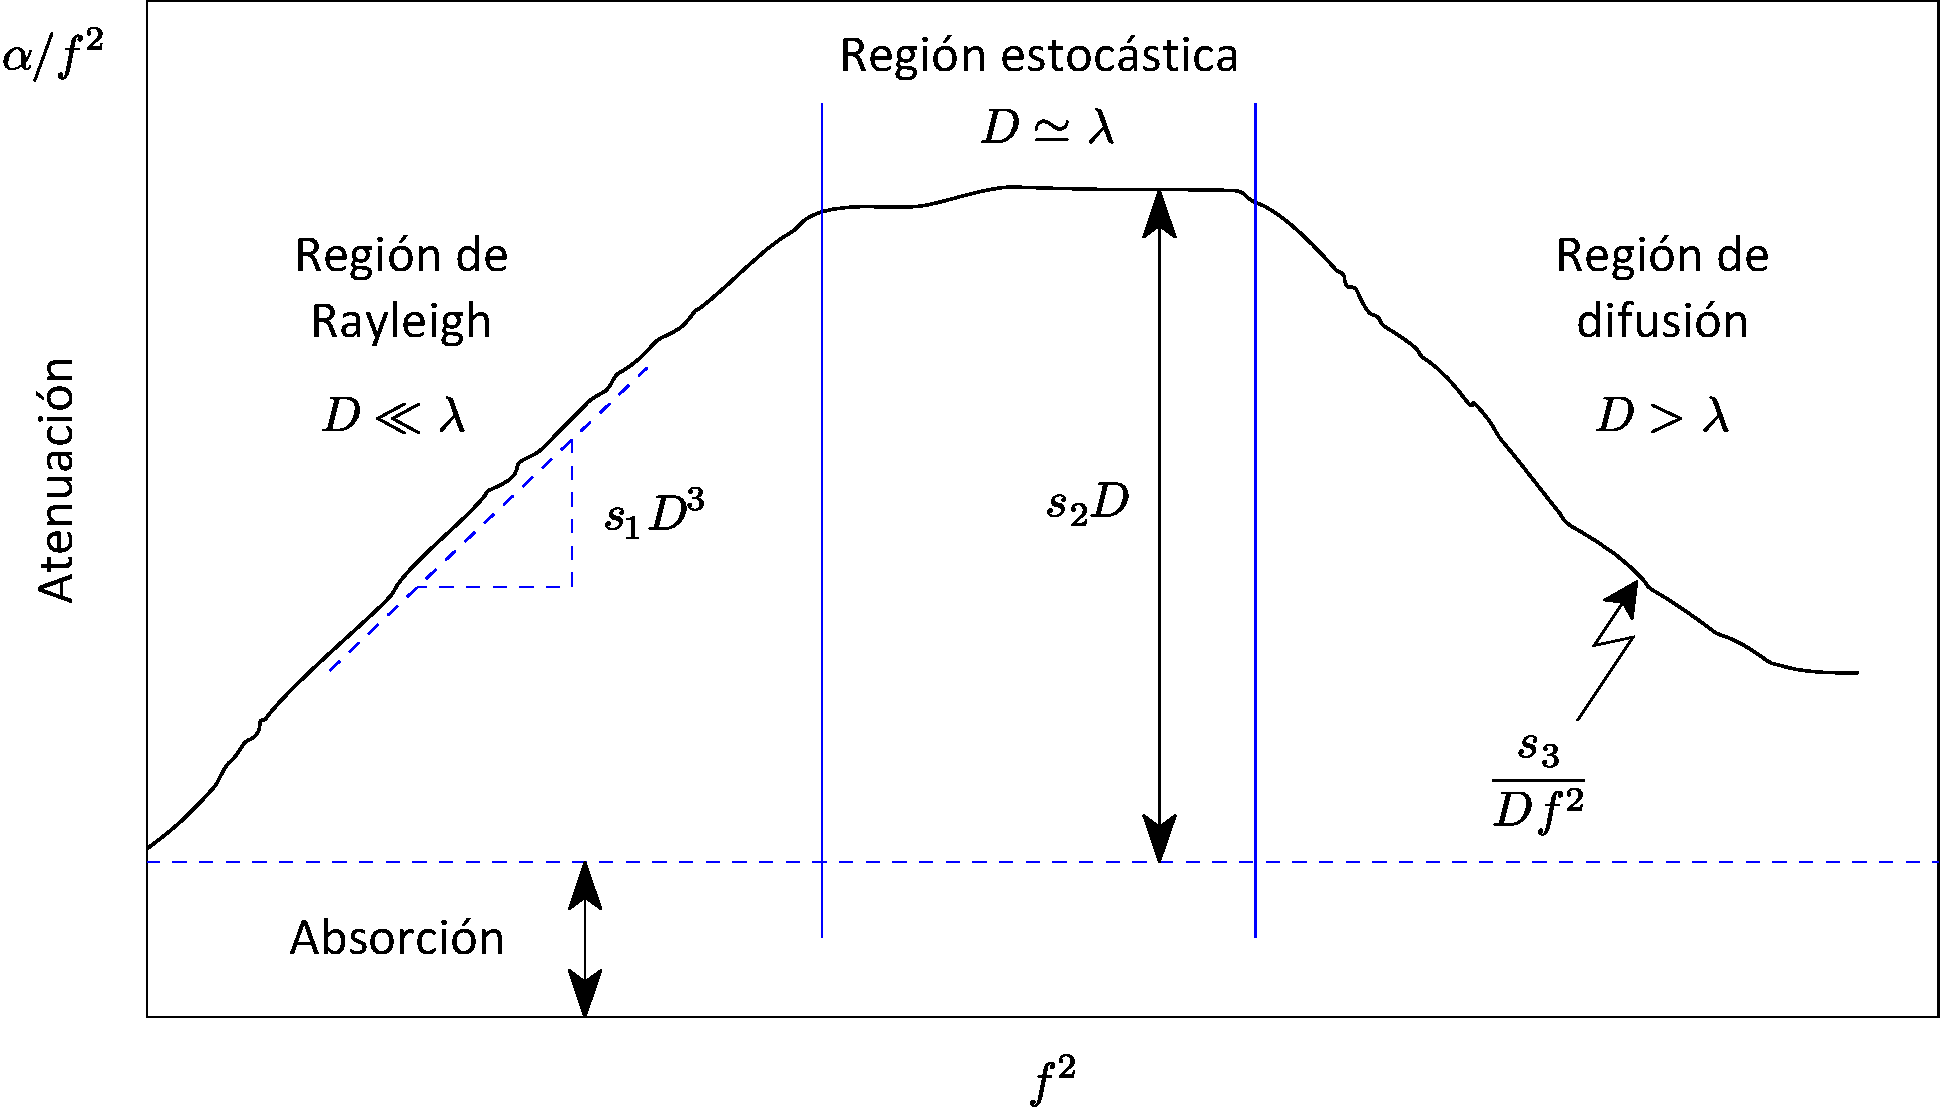
\includegraphics{gis-pfc-ch3-06.mps}
	\end{center}
	\caption[Dos líneas de prueba]{Dos líneas de texto de prueba para
	comprobar como cambia la estructura del documento si lo comprimo un
	poquito.}
% 	\caption[Modo de funcionamiento continuo]{La ventana temporal %
% 	tiene, en este ejemplo, una duración de cinco ventanas de %
% 	adquisición. Al llegar al sistema el sexto fragmento de señal, la %
% 	representación avanza a la derecha retirándose el primer fragmento %
% 	representado para dar cabida al fragmento obtenido recientemente.}
	\label{fig:modcontii}
\end{figure}

La alta tasa con la que aparecen las imágenes por pantalla garantizan que
la representación siga casi en tiempo real ---por lo menos así lo percibe
el ojo humano--- a la señal verdadera. Debe notarse, no obstante, que este
método de representación no es adecuado para señales de alta frecuencia
pues aunque el eje temporal abarque un tiempo mayor, la dimensión del
monitor obviamente no varía y las señales de alta frecuencia aparecerán en
exceso comprimidas.


\subparagraph{Modo convencional}

El \emph{modo convencional} de representación es algo más complicado. La
representación convencional basa su funcionamiento en imágenes que muestran
fragmentos de señal que cubren la dimensión temporal de la ventana del
osciloscopio y que se suceden unas a otras con presteza. La idea que
persigue este método es la de conseguir algo semejante a una película de la
señal. Para ello, no es sólo suficiente con que aparezcan muchas imágenes
por segundo en el monitor del osciloscopio, esas imágenes deben estar de
algún modo relacionadas entre sí. Si las imágenes que aparecen en el
monitor son de forma consecutiva muy diferentes es probable que no pueda
discernirse nada claro, y en ese caso de nada vale la representación.

Ahí es donde entra en juego el procesado y la función de disparo de un
osciloscopio digital. Cuando un fragmento suficientemente largo como para
cubrir la ventana de representación se digitaliza y se almacena en memoria,
empieza el procesado digital del mismo. El propósito del procesado es, ente
otras cosas, eliminar las posible componente en continua, averiguar
información adicional de la señal en la medida de lo posible, como p. ej.
su valor de pico a pico, o implementar la función de disparo. La función de
disparo del osciloscopio persigue alinear los ejes verticales de la ventana
donde se representa con los cruces de la señal con respecto a un
determinado valor de umbral que puede ser configurado por el usuario. La
idea es alinear al menos el cruce más centrado de cada fragmento de señal
con el eje de abscisas que corta en dos mitades la ventana. Para
conseguirlo, durante el procesado se detectan todos los cortes de la señal
con el umbral y después se desplaza el fragmento de señal para que el corte
más centrado case con el eje de abscisas. Si la señal es periódica las
variaciones entre un fotograma y el siguiente serán mínimas, puesto que
ambos estarán alineados, y se simulará con éxito el movimiento.

No obstante, la necesidad de desplazar el fragmento de señal que va a
representarse presenta un inconveniente importante. Para poder desplazar el
fragmento de señal y que se cubra completamente la ventana del osciloscopio
su duración debe ser superior al tiempo reflejado en el eje de tiempos de
la ventana. De lo contrario la señal aparecerá truncada, se mostrará un
espacio en blanco y con una tasa de refresco alta la visualización será
confusa. Desplazar fragmentos de señal implica dos cosas: por un lado el
osciloscopio debe esperar más tiempo para refrescar la pantalla, es decir,
se reduce la tasa de refresco para una misma configuración del eje de
tiempos; y por otro, al tener para representar un fragmento de señal de
mayor duración que la reflejada por el eje temporal de la ventana parte del
fragmento queda ahora fuera de la representación.

Este inconveniente se ve paliado por el hecho de que el modo convencional
contempla en principio trabajar con señales de alta frecuencia. Estas
señales cambian de forma tan rápida que de no ser por el disparo sería
imposible observar los cambios. Por otro lado puede seleccionarse que
información que se muestra por pantalla accionando un control de
desplazamiento temporal o modificando el valor de umbral de disparo y,
generalmente, la pérdida de información a causa del disparo no es
significativa.

Para terminar este apartado se han adjuntado las
\cref{fig:freesignaltrig,fig:modtrig} que muestran los distintos aspectos
del modo disparado de funcionamiento del osciloscopio que se han expuesto
aquí. La \cref{fig:freesignaltrig} muestra la señal que entra al sistema,
se han marcado los instantes en los que se suceden los eventos más
relevantes en la representación de un fragmento de señal. También se
muestran el nivel de umbral y la porción de fragmento de señal que coincide
con las muestras descartadas. Otra figura, la \cref{fig:modtrig} muestra
cual es el resultado de representar el fragmento de señal en la ventana del
osciloscopio.

\begin{figure}
	\begin{center}
		\includegraphics{gis-pfc-ch3-02.mps}
	\end{center}
	\caption[Fragmento de señal adquirido por el osciloscopio en el
	espacio de una ventana de adquisición]{Fragmento de señal adquirido
	por el osciloscopio en el espacio de una ventana de adquisición. En
	esta figura se ha representado también la duración de la ventana
	temporal del osciloscopio, pudiendo observarse que información se
	descarta. También se indica el instante en el que se inicia una
	nueva instancia del proceso de adquisición, de lo que puede
	deducirse que información se pierde entre instancias. Los cortes de
	la señal con el nivel de disparo también están representados.}
	\label{fig:freesignaltrig}
\end{figure}

\begin{figure}
	\begin{center}
		\includegraphics{gis-pfc-ch3-03.mps}
	\end{center}
	\caption[Modo de funcionamiento disparado]{Modo de funcionamiento
	disparado. La representación se centra en el corte central (veáse
	la \vref{fig:freesignaltrig}).}
	\label{fig:modtrig}
\end{figure}


\section{Elaboración del software de control}


\subsection{Elección del entorno de desarrollo}\label{subsec:environment}

El lenguaje o, mejor dicho, plataforma que se ha empleado para el
desarrollo del software de control es \matlab{}, la razón, su inmejorable
compatibilidad con el hardware disponible. A partir de ahí, los componentes
de \matlab{} que se han empleado para conseguir que el software de control
gozase de las características previstas en la etapa de diseño son dos: el
entorno de desarrollo de interfaces gráficas de usuario (\emph{Graphical
user interface}, en lo sucesivo \psig{gui}) de \matlab{}, más conocido como
\psig{guide} (\emph{Graphical user interface development environment}); y
la herramienta de adquisición de datos de \matlab{} (\emph{Data acquisition
toolbox}, en adelante \psig{DAT}) . El primero de ellos se ha empleado
para, como su nombre indica, crear la interfaz que comunica el dispositivo
con el usuario. Esta comunicación se hace a través del segundo de los
componentes mencionados, éste permite, mediante comandos de \matlab{} que
pueden incluirse en rutinas o llamarse por separado, manejar el dispositivo
---convocarlo a muestrear, configurar sus propiedades--- y administra
automáticamente los resultados almacenándolos en búffers situados en la
memoria volátil del ordenador, haciéndolos de este modo accesibles al
administrador de la tarjeta.


\subsection{Data Acquisition Toolbox}

La práctica de emplear \gui{} como fondo para aplicaciones desarrolladas
con \matlab{} es bastante habitual, así como lo es programar esas
interfaces mediante \guide{}. Por ello, y dado que la documentación que se
ciñe a tratar la problemática que envuelve esta actividad es abundante, se
ha preferido dejar a cargo de dichos documentos este asunto y centrar este
escrito en presentar con concisión los principios necesarios para emplear
con éxito la \datx{} de \matlab{} en el manejo de dispositivos para la
adquisición de señales analógicas. La fórmula elegida con tal propósito
consiste en describir cual es el procedimiento habitual en una sesión de
adquisición de datos y en cada paso detallar las opciones más
significativas y proporcionar ejemplos explicativos extraídos del mismo
código que integra el software de control.

En cuanto a la documentación adicional que el lector puede consultar a
continuación se citan varios documentos clasificados en función del tema
que tratan. Para la programación de \gui{} con \matlab{} puede consultarse
el manual de usuario, cite, disponible en la web del fabricante. Esta
sección se basa en la guía rápida sobre el uso de la \datx{}, también a
cargo de \emph{The MathWorks, Inc.}, la compañía que mantiene la suite
matemática en cuya web puede obtenerse un documento extendido.


\subsubsection{Componentes de la herramienta}

Los elementos de \matlab{} que juegan un papel suficientemente importante
en el funcionamiento de la \datx{} son los listados en el
\cref{tab:toolcomp}. El diagrama representado en la \vref{fig:toolcomp}
muestra las interdependencias que existen entre los elementos que aparecen
en dicho cuadro.

\begin{table}
	\centering
	\begin{tabulary}{.9\textwidth}{C L}
		\toprule
		Componente & \multicolumn{1}{c}{Propósito} \\
		\midrule
		Ficheros *.m & Se emplean para automatizar la creación de
		objetos dispositivo, adquirir datos, configurar las
		propiedades del dispositivo y la sesión, y evaluar el
		estado de la adquisición y los recursos.\\
		\midrule
		Máquina virtual de adquisición de datos & Almacena objetos
		dispositivo y sus propiedades, controla el almacenamiento
		de los datos adquiridos y controla la sincronización de
		eventos.\\
		\midrule
		Adaptadores & Son la vía de comunicación entre la máquina
		virtual de adquisición de datos y el hardware por la cual
		se transmiten propiedades, datos y eventos.\\
		\bottomrule
	\end{tabulary}
	\caption[Descripción de los componentes de la \datx{}] {Descripción
	de los componentes de la \datx{}.}
	\label{tab:toolcomp}
\end{table}

\begin{figure}
	\begin{center}
		\includegraphics{gis-pfc-ch3-07.mps}
	\end{center}
	\caption[Elementos que intervienen en el funcionamiento de la
	\datx{}]{Elementos que intervienen en el funcionamiento de la
	\datx{}.}
	\label{fig:toolcomp}
\end{figure}

\subsubsection{Objetos dispositivo}

Los objetos dispositivo permiten el acceso a subsistemas específicos del
hardware. Los objetos dispositivo soportados por la \datx{} son los objetos
de entrada analógica o \emph{analog imput objects} (\psig{ai}), los objetos
de salida analógica o \emph{analog output objects} (\psig{ao}) y los
objetos de entrada/salida digital o \emph{digital I/O objects}
(\psig{dio}).

\begin{figure}
	\begin{center}
		\includegraphics{gis-pfc-ch3-08.mps}
	\end{center}
	\caption[Comunicación entre los subsistemas del hardware y los
	objetos dispositivo]{Grafo que representa la comunicación entre los
	subsistemas del hardware y los objetos dispositivo.}
	\label{fig:subsystemsOO}
\end{figure}


\subsection{La sesión de adquisición de datos}

Una sesión completa de adquisición de datos consiste en cinco pasos:

\begin{enumerate}
	\item Crear el objeto dispositivo.
	\item Añadir canales al objeto dispositivo.
	\item Configurar las propiedades del objeto dispositivo y los
		canales añadidos para controlar el comportamiento de la
		aplicación de adquisición de datos.
	\item Adquirir los datos.
	\item Eliminar el objeto dispositivo.
\end{enumerate}

Cada uno de los pasos se detalla en los puntos subsiguientes.


\subsubsection{Crear el objeto dispositivo}

Para crear un objeto dispositivo, se debe llamar a la función de creación
apropiada o constructor. Como se muestra en el \cref{tab:constructors}, los
constructores reciben un nombre particular en función del tipo de objetos
dispositivo que crean. Para iniciar una sesión de adquisición de datos
analógicos es necesario un comando como el siguiente,
\func{analoginput(`adaptador', ID)}. Un ejemplo extraído del código fuente
de la aplicación de control muestra cómo hacerlo en el
\cref{cod:constructor}.

\begin{table}
	\centering
	\begin{tabular}{l >{\tt}l}
		\toprule
		\multicolumn{1}{c}{Tipo de subsistema} %
		& \multicolumn{1}{c}{\rm Constructor} \\
		\midrule
		Entrada analógica & analoginput(`adaptador', ID); \\
		\midrule
		Salida analógica & analogoutput(`adaptador', ID); \\
		\midrule
		Entrada / Salida digital & digitalio(`adaptador', ID); \\
		\bottomrule
	\end{tabular}
	\caption[Tipos de constructor en función del objeto dispositivo
	creado]{Tipos de función de creación de acuerdo con el tipo
	subsistema al que se orienta el objeto dispositivo creado.}
	\label{tab:constructors}
\end{table}

\begin{lstlisting}[style=displayed, caption={[Método a seguir para crear un
	objeto dispositivo] {Método que evalúa la existencia de un objeto
	dispositivo previo a la llamada de la aplicación, en caso positivo
	lo hereda para su uso posterior, de lo contrario crea uno
	nuevo.}}, label={cod:constructor}]
	set(handles.ai, 'TriggerType', 'Immediate', 'TimerFcn', '', ...
	handles.ai = [];

	if ~isempty(daqfind)
		oldObj = daqfind;

		for i = 1:length(oldObj);
			auxStr = daqhwinfo(oldObj(i));
			auxNum = findstr(' ', auxStr.DeviceName) - 1;
			if strcmp('KPCI-3108', ...
				auxStr.DeviceName(1:auxNum)) && ...
				strcmpi('analoginput', auxStr.SubsystemType);
				handles.ai = oldObj(i);
				warning('El dispositivo esta en uso.');
				break
			end
		end

	end

	if isempty(handles.ai)
		try
			handles.ai = analoginput('keithley');
		catch
			errordlg('No pudo crearse el manejador de dispositivo.');
		end
	end
\end{lstlisting}

El argumento \func{id} es un indicador de dispositivo hardware. Se trata de
un argumento opcional para tarjetas de sonido con \func{id} 0. El argumento
\func{adaptador} requiere el nombre del adaptador de dispositivo hardware.
A continuación, en el \cref{tab:adaptors} se muestra una relación con los
adaptadores de dispositivo cuyo uso es más frecuente y el nombre de
adaptador que debe introducirse como argumento de la llamada a
\func{analoginput}. Por conveniencia se ha añadido Keithley a esta lista.

\begin{table}
	\centering
	\begin{tabular}{l >{\tt\qquad}l}
		\toprule
		\multicolumn{1}{c}{Fabricante de Hardware} %
		& \multicolumn{1}{c}{\rm Nombre de adaptador} \\
		\midrule
		Advantech & advantech \\
		\midrule
		Measurement Computing & mcc \\
		\midrule
		National Instruments & nidaq \\
		\midrule
		Parallel port & parallel \\
		\midrule
		Microsoft Windows & winsound \\
		\midrule
		Keithley Instruments, Inc. & keithley \\
		\bottomrule
	\end{tabular}
	\caption[Argumento que debe emplearse en la llamada a
	\func{analoginput} en función del fabricante]{Argumento que debe
	emplearse en la llamada a \func{analoginput} en función del
	fabricante.}
	\label{tab:adaptors}
\end{table}


\subsubsection{Añadiendo canales}

Antes de poder utilizarse, deben añadirse canales al objeto dispositivo.
Para ello, debe emplearse la función \func{addchannel}. Puede pensarse en
un objeto dispositivo como un contenedor de grupos de canales y en los
canales añadidos a un objeto dispositivo como un grupo de canales. Si se
desean añadir dos canales al objeto dispositivo \func{objeto} puede
utilizarse la siguiente llamada \func{cans = addchannel(objeto, 1:2);}.


\subsubsection{Configurando propiedades}

Puede controlarse el comportamiento de una sesión de adquisición de datos o
de una aplicación creada con tal propósito configurando las propiedades de
los objetos dispositivo que intervienen en el proceso de adquisición y de
los canales que dicho objeto contiene. Estas son las reglas principales en
la configuración de propiedades desde la \datx{}.

\begin{itemize}
	\item Los nombres de las propiedades pueden escribirse en
		mayúsculas, minúsculas o combinación de ambas.
	\item Los nombres de las propiedades pueden abreviarse como se
		mostrará a continuación. % Hay que confirmar que se
		% explican las reglas de abreviatura
	\item La función \func{set} aplicada a un objeto dispositivo
		---\func{set(objeto)}--- devuelve todas las propiedades
		configurables de ese objeto. Si se llama a \func{set}
		utilizando como argumento un canal
		---\func{set(objeto.Channel(índice)}---, la función
		devolverá todas las propiedades configurables de dicho
		canal.
	\item La función \func{get} devuelve todas las propiedades de un
		canal u objeto y el valor que toman en el momento en el que
		se llama a la función si se emplea como único argumento
		dicho canal u objeto ---\func{get(objeto)}, \\
		\func{get(objeto.Channel(índice)}---.
\end{itemize}

Se distinguen dos tipos de propiedades distintas asociadas a los canales
contenidos en un objeto dispositivo.

\begin{description}
	\item[Propiedades comunes] Son aquellas propiedades que se aplican
		todos los canales pertenecientes a un mismo objeto
		dispositivo.
	\item[Propiedades de canal] A diferencia de las propiedades
		comunes, las propiedades de canal pueden configurarse
		individualmente por canal.
\end{description}

Dentro de las propiedades comunes de los canales existen las
\emph{propiedades básicas}, que se aplican a todos los subsistemas de un
determinado tipo (\textsc{ai, ao, dio}); y \emph{propiedades específicas de
dispositivo} aplicables únicamente al hardware específico que se está
empleando.

Existen tres formas de configurar u obtener el valor de una propiedad:
utilizando las funciones \func{set} y \func{get}; empleando la notación de
punto; o recurriendo a los nombres indexados.

\begin{itemize}
	\item La sintaxis de las funciones \func{get} y \func{set} es
		similar a la empleada en la herramienta de \matlab{}
		\emph{Handle Graphics}.

		\begin{lstlisting}[gobble=16]
			out = get(objeto, `SampleRate');
			set(objeto, `SampleRate', 11025)
		\end{lstlisting}

	\item La notación de punto se emplea del siguiente modo:

		\begin{lstlisting}[gobble=16]
			out = objeto.SampleRate;
% 			objeto.SampleRate = 11025;
		\end{lstlisting}

	\item Por último, los nombres indexados permiten asociar un nombre
		descriptivo a cada canal. Por ejemplo para asociar el
		nombre \func{Can1} con el primer canal contenido en
		\func{objeto} debe procederse como se enuncia a
		continuación.

		\begin{lstlisting}[gobble=16]
			set(objeto.Channel(1), `ChannelName', `Can1');
			out = objeto.Can1.UnitsRange;
			objeto.Can1.UnitsRange = [0, 10];
		\end{lstlisting}

\end{itemize}


\subsubsection{Adquisición de datos}

La adquisición de datos puede dividirse en tres tareas básicas: iniciar el
objeto dispositivo; registrar datos y detener el objeto dispositivo.

La función que se utiliza para iniciar un objeto dispositivo es la función
\func{start}, p.e. para iniciar el objeto dispositivo \func{objeto} habría
que llamar a la función de esta forma \func{start(objeto)}. Tras iniciar un
objeto su propiedad \textsf{Running} pasa de manera automática al valor
\textsf{On}.

No obstante haber iniciado el dispositivo, este no empieza a registrar
datos hasta que no ocurre un trigger o disparo. Hay diversos tipos de
trigger, en el \vref{tab:triggers} se muestran aquellos soportados por
todos los dispositivos. Tras un trigger el dispositivo hardware inicia la
adquisición de datos y la propiedad \textsf{Logging} del objeto dispositivo
asociado conmuta al estado \textsf{On}.

\begin{table}
	\centering
	\begin{tabulary}{.9\linewidth}{>{\sf}c L}
		\toprule
		{\rm Tipo de disparo} & \multicolumn{1}{c}{Descripción} \\
		\midrule
		Inmediato & El disparo ocurre justo después de la llamada a
		\func{start}. Este es el tipo de trigger predeterminado. \\
		\midrule
		Manual & El disparo ocurre después de llamar manualmente a
		la función \func{trigger}. \\
		\midrule
		Software & El disparo sucede cuando se detecta una señal
		que satisface una determinada condición especificada de
		antemano. El objeto dispositivo debe disponer de más de un
		canal que hará las veces de la señal de disparo. Debe
		especificarse, como es obvio, que canal actúa como fuente
		del disparo. \\
		\midrule
		Reloj interno & Por añadidura, la \kpci{} cuenta con la
		posibilidad de recibir el disparo de la fuente de reloj
		interna. \\
		\bottomrule
	\end{tabulary}
	\caption[Tipos de disparo soportados por el hardware compatible con
	\matlab{}]{Tipos de disparo soportados por el hardware compatible
	con \matlab{} y una breve descripción de los mismos.}
	\label{tab:triggers}
\end{table}

Por último, existen tres causas por las que un objeto dispositivo puede
detenerse: \matlab{} detiene un objeto dispositivo iniciado una vez
obtenidos los datos precisados por el usuario; al ocurrir un error de
tiempo de ejecución en relación con la actividad de un objeto dispositivo
éste es detenido también; y tan sólo resta el método manual, que consiste
en llamar a la función \func{stop}, por ejemplo \func{stop(objeto)}.

Como se ha mencionado la máquina virtual de adquisición de datos registra y
controla los datos que extrae de un objeto dispositivo. Un usuario puede
acceder a esos datos de dos formas diferentes:

\begin{itemize}
	\item La primera de ellas se conoce como previsualizar los datos.
		Se emplea con ese propósito la función \func{peekdata}. Si,
		por ejemplo, se quisiese previsualizar 1000 muestras
		obtenidas con el objeto dispositivo \func{objeto}, la
		llamada a \func{peekdata} sería la siguiente: \func{out =
		peekdata(objeto, 1000);}. La función \func{peekdata}
		devuelve el control a \matlab{} de inmediato y no elimina
		los datos previsualizados de la máquina virtual de
		adquisición.
	\item En cualquier momento tras adquirir datos mediante un objeto
		dispositivo estos pueden extraerse de la máquina virtual de
		adquisición mediante la función \func{getdata}. Partiendo
		del ejemplo anterior, si se desea extraer 1000 muestras
		procedentes del objeto dispositivo \func{objeto}, esta es
		la llamada adecuada \func{out = getdata(objeto, 1000);}. Al
		contrario que la función \func{peekdata}, \func{getdata} no
		devuelve el control a \matlab{} hasta haber extraído todas
		las muestras solicitadas. Es evidente que las muestras
		extraídas dejarán de estar disponibles en la máquina
		virtual de adquisición.
\end{itemize}

Es importante señalar que en cualquiera de los procedimientos descritos
intentar acceder a más datos de los obtenidos en un determinado momento
causará un error que detendrá el funcionamiento del objeto dispositivo.


\subsubsection{Eventos y Callbacks}

Puede decirse que un evento sucede en un determinado instante después de
que una cierta condición se cumple. A menos que ocurra un error, en todas
las sesiones de adquisición de datos debe producirse un evento de inicio,
uno de disparo y uno de parada. Puede accederse a la información que
transporta un evento mediante la propiedad \textsf{EventLog}:

\begin{lstlisting}
	Events = ai.EventLog;
	EventTypes = {Events.Types}
	EventTypes =
		`Start'    `Trigger'	`Stop'
\end{lstlisting}

Cuando se produce un evento, puede ejecutarse una función de
\emph{callback}. Es posible seleccionar una función para un callback
especificando como valor de la propiedad asociada a dicho callback el
nombre de la función (si ésta se encuentra en el mismo fichero *.m que
contiene el código que ejecuta la aplicación que realiza la adquisición de
datos), o el nombre del fichero *.m con el código de la función. Así mismo,
pueden pasarse argumentos de entrada a la función de callback asignándolos
a la mencionada propiedad.

Por ejemplo, los siguientes comandos configuran \func{objeto} de forma que
la función \func{datadqcallback} se ejecute desde el fichero cuyo nombre
está compuesto por una raíz idéntica al nombre de la función y con
extensión *.m, cuando se produzca un evento de trigger o de parada durante
la actividad del objeto dispositivo. Además se pasa como argumento de la
función el valor de la propiedad \textsf{Running} de \func{objeto} en el
momento del callback.

\begin{lstlisting}
	set(objeto, `TriggerFcn', @datadqcallback, objeto.Running)
	set(objeto, `StopFcn', @datadqcallback, objeto.Running)
\end{lstlisting}

Un segundo ejemplo, este extraído del código fuente de la aplicación de
control muestra como pasar argumentos a la función de callback y cuál es la
sintaxis de la definición de la misma en el \cref{cod:callback}.

\begin{lstlisting}[style=displayed, caption={[Configuración de
	\emph{callback}]{Configuración de \emph{callback} para responder a
	eventos en la sesión de muestreo, la función de \emph{callback}
	recibe un argumento.}}, label={cod:callback}]
	set(handles.ai, 'TriggerType', 'Immediate', 'TimerFcn', '', ...
		'SamplesAcquiredFcn', {@localDaqCallback, gcbo});

				[...]

	function localDaqCallback(obj, event, hObject)
		handles = guidata(hObject);
		EventType = event.Type;

		switch lower(EventType)
			case 'samplesacquired'

				[...]

			case 'timer'

				[...]

		end
\end{lstlisting}

\subsubsection{Suprimiendo y borrando las trazas de los objetos dispositivo}

La función \func{delete} elimina el objeto dispositivo especificado de la
máquina virtual de adquisición, pero no del espacio de trabajo de
\matlab{}, ---\func{delete(objeto)}---. Tras una llamada semejante
\func{objeto} sigue apareciendo en el espacio de trabajo de \matlab{}, pero
se trata de un objeto inválido desde el momento en el que deja de
encontrarse ligado al hardware. Deben suprimirse los objetos dispositivo
faltos de validez con el comando \func{clear}, p.e., \func{clear
objeto}.

Si se suprime un objeto dispositivo del espacio de trabajo de \matlab{} no
deja de existir en la máquina virtual. Para poder recuperar objetos
borrados accidentalmente puede utilizarse la función \func{daqfind}.

\begin{lstlisting}
	out = daqfind;	ai = out(1);
\end{lstlisting}
